
\section{Numerical results}
\subsection{Hertz’s half-idsks}
\begin{frame}\frametitle{Numerical results}
	\textbf{\bl{Hertz’s half-disks problem}}
	\begin{itemize}
		\item Imposed displacement on the upper half-sphere
		\item Parametric radius $\mu$ for the lower half-sphere
		% \item $E = 15$Pa, $\nu=0.35$,
		\item $\mathcal P = [0.9, 1.12]$, $\mathcal P^{\rm tr} = \{0.905+0.01i | \ 0\leq i\leq 22\}$
		\item Non-matching meshes, $\mathcal N = 1350$ nodes, $\mathcal R = 51$
	\end{itemize}
	\hspace{-0.5cm}
	\mbox{
		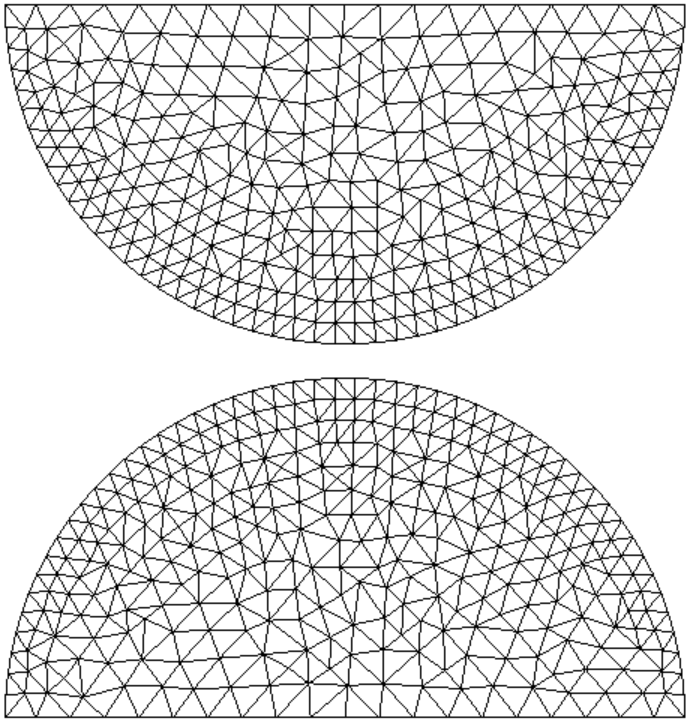
\includegraphics[width=0.35\textwidth]{./images/contact/ref_config.png}
		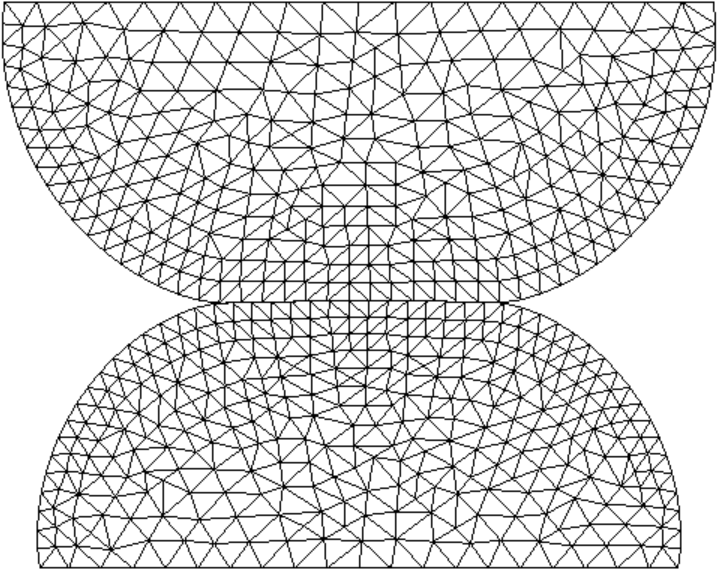
\includegraphics[width=0.35\textwidth]{./images/contact/contact_09.png}
		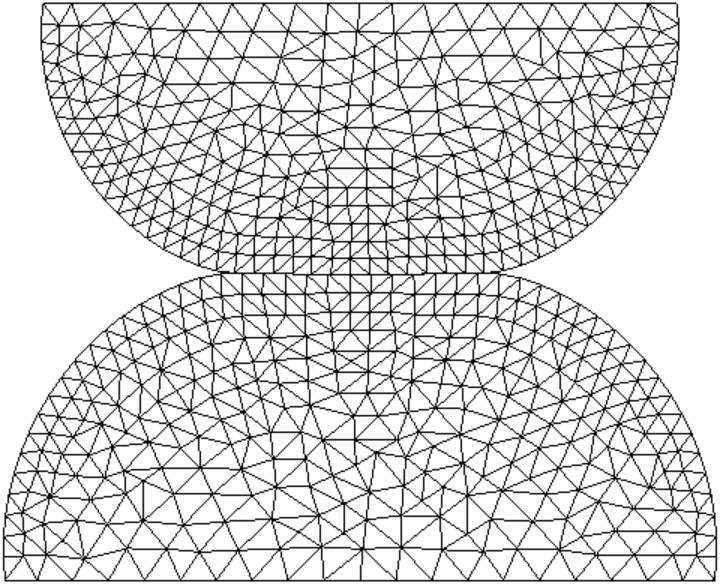
\includegraphics[width=0.38\textwidth]{./images/contact/contact.png}
	}
	\vspace{-0.3cm}
	\hspace{-0.2cm}
	Reference configuration 
	\qquad\qquad $\mu = 0.9$
	\hspace{3cm} $\mu = 1.12$
\end{frame}


\begin{frame}\frametitle{High-fidelity solution procedure}
	\vspace{-0.2cm}
	\small{
		\begin{itemize}
			\item \bl{Conforming FEM for displacement,}\ma{dG $\mathbb P_0$ for contact pressures}
			\begin{itemize}
				\item \ma{Collocation}at contact nodes (possible instability)
				\item Local Averaged Contact \ma{(LAC)}: macro-elements (two consecutive segments) \gr{(Drouet, Hild ('17))}
			\end{itemize}
		\end{itemize}
	}
	\vspace{-.25cm}
	\begin{center}
		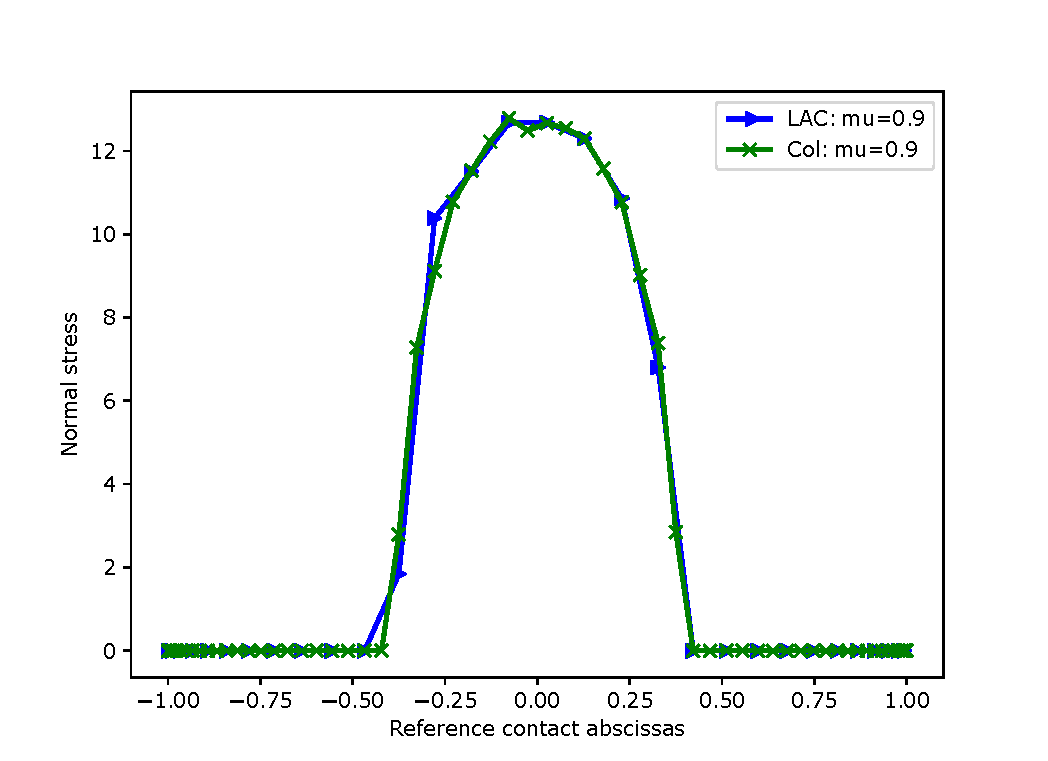
\includegraphics[width=.35\textwidth]{./images/contact/nn61_mu=0,9_iters_LAC_20_colloc_24.pdf} \qquad
		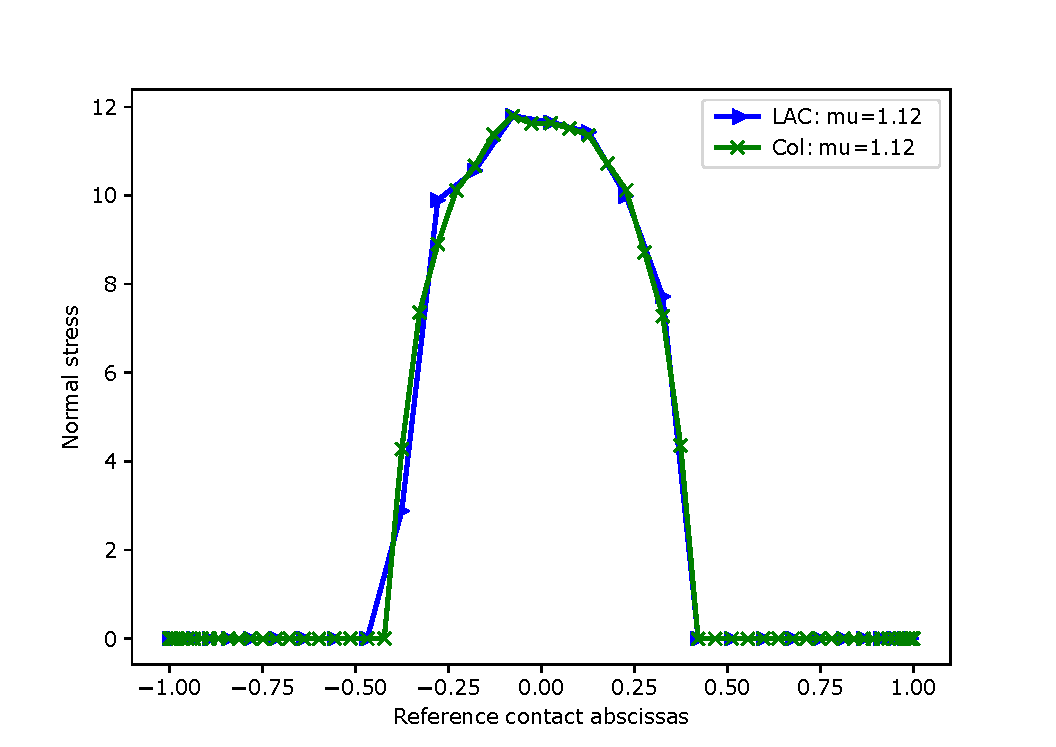
\includegraphics[width=.35\textwidth]{./images/contact/nn61_mu=1,12_iters_LAC_18_colloc_24.pdf} \\[-3pt]
		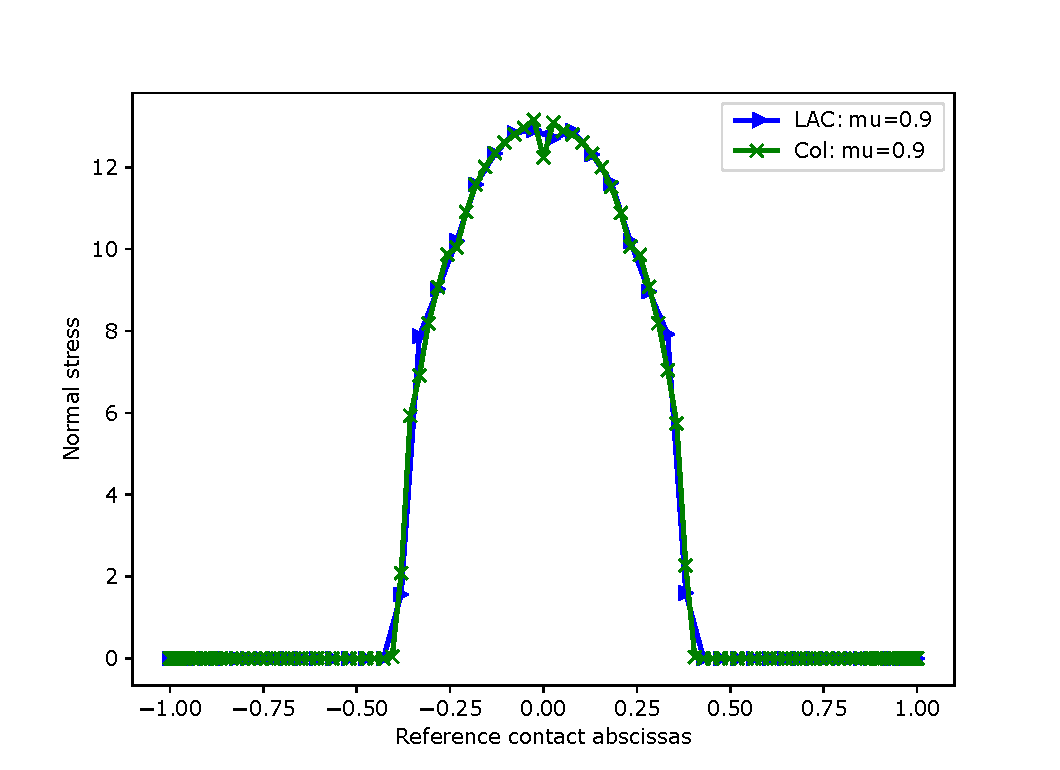
\includegraphics[width=.35\textwidth]{./images/contact/nn121_mu=0,9_iters_LAC_27_colloc_28.pdf} \qquad
		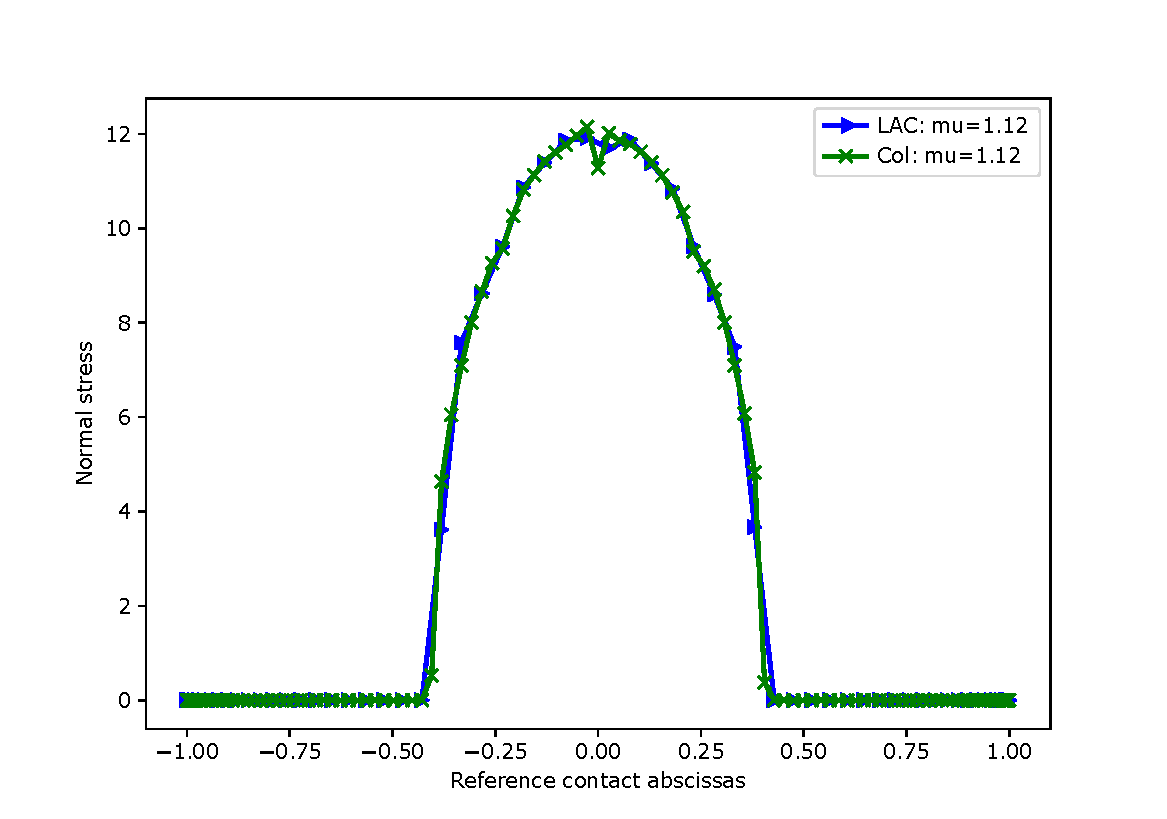
\includegraphics[width=.35\textwidth]{./images/contact/nn121_mu=1,12_iters_LAC_20_colloc_25.pdf} \\
		\tiny{$\mu=0.9$ (left) / $1.12$ (right), coarse (top) / fine (bottom) meshes}
	\end{center}
\end{frame}


\begin{frame}\frametitle{Basis constructions}
	% \vspace{-0.15cm}
	% Primal basis dimension $N$ as a function of the truncation threshold $\epsilon_{\rm pod}$
	% \vspace{-0.15cm}
	% \begin{table}[htb]
		% \centering
		% \begin{tabular}{|c||c|c|c|c|c|c|}
			% \hline
			%       $\epsilon_{\rm pod}$ &$10^{-2}$ & $10^{-3}$ & $10^{-4}$ &$10^{-5}$ \\ \hline
			%       $N$ &
			%       $5$& $11$ & $16$ & $20$\\ \hline
			%       	\end{tabular}
		% \label{tab:sgv}
		% \end{table}
	
	% \vspace{-0.2cm}
	
	\hspace{-1.1cm}
	\begin{minipage}{\textwidth}
		\begin{figure}
			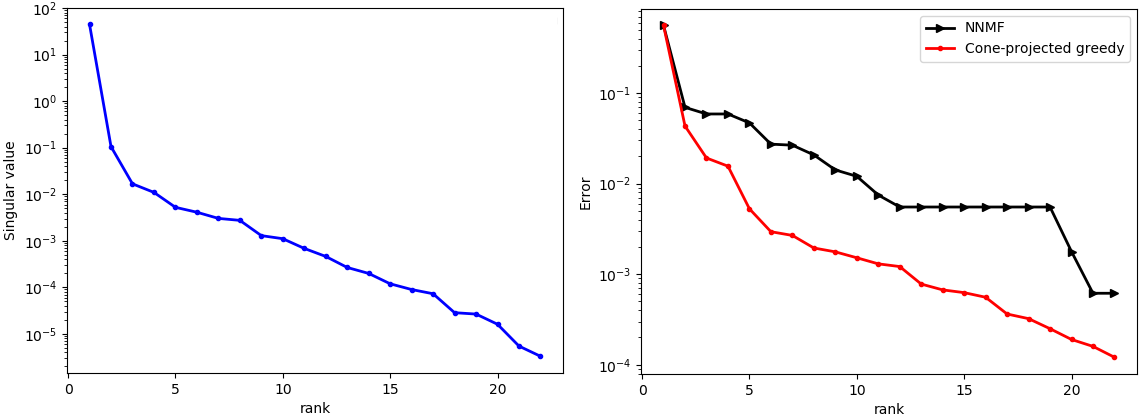
\includegraphics[width=1.18\textwidth]{./images/contact/sgv_nmf.png}
			\centering
			\tiny{\white{jvjhkhjndscccxcvvwlklkiu}Primal POD basis \hspace{5cm} Dual basis
			}
			\centering
		\end{figure}
	\end{minipage}
	
	\bigskip 
	
	Dual basis dimension $R$ as a function of the truncation threshold $\epsilon_{\rm du}$
	\vspace{-.1cm}
	\begin{table}[htb]
		\centering
		\begin{tabular}{|c|c||c|c|c|c|c|}
			\hline
			\multicolumn{2}{|l||}{\qquad\qquad\quad$\epsilon_{\rm du}$} &$5\cdot10^{-2}$ & $10^{-2}$ & $5\cdot10^{-3}$ &$10^{-3}$\\ \hline
			{NMF}&$R$ &
			$4$ & $10$ & $19$ & $20$\\ \hline
			{Cone-projected greedy}&$R$ &
			\bl{$2$}& \bl{$5$} & \bl{$6$} & \bl{$13$}\\ \hline
		\end{tabular}
		\label{tab:nmf}
	\end{table}
\end{frame}

\begin{frame}\frametitle{Empirical interpolation}
	EIM error as a function of the rank $M$ of the EIM approximation.
	\medskip
	
	\begin{figure}[ht!]
		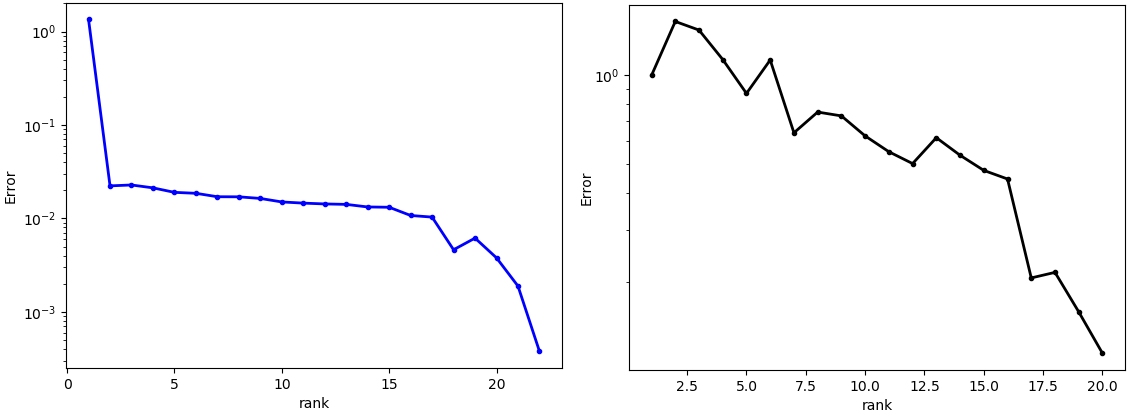
\includegraphics[width=\textwidth]{./images/contact/eims.png}
		\centering 
		\tiny{\white{waalou}Nonlinear gap map $\mathbf g(\mu,\mathbf u(\mu))$\white{rien de rien, je ne re}
			Nonlinear contact map $\mathbf K(\mu,\mathbf u(\mu))$}
	\end{figure}
	% $\epsilon_{\rm du}=10^{-4}$, $\epsilon_{\rm eim}^k=10^{-2}$, $\epsilon_{\rm eim}^g=10^{-3}$ and $\epsilon_{\rm pod}=10^{-5}$.
\end{frame}

\begin{frame}\frametitle{Error estimation}
	% Error indicators
	% \begin{align*}
		% &e_{\rm ener}(\mu):= \frac{1}{2}|a(\mu,\widehat u(\mu),\widehat u(\mu))-f(\mu,\widehat u(\mu))-a(\mu,u(\mu),u(\mu))+f(\mu,u(\mu))|,\\
		% &e_{\rm displ}(\mu):=\frac{\|\widehat u(\mu)-u_\mathcal N(\mu)\|_{H^1(\Omega^{\rm tr})}}{\|u_\mathcal N(\mu)\|_{H^1(\Omega^{\rm tr})}}.
		% \end{align*}
	\hspace{-1.05cm}
	\begin{minipage}{\textwidth}
		\begin{figure}[ht!]
			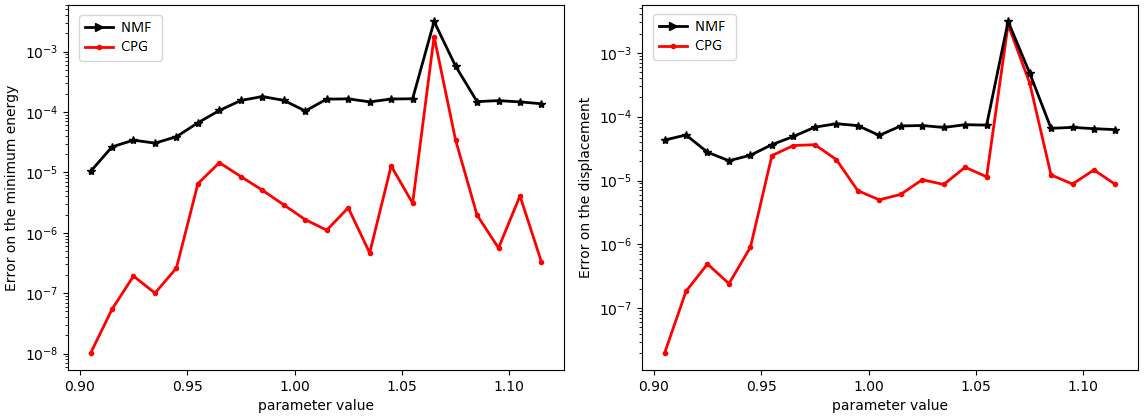
\includegraphics[width=1.17\textwidth]{./images/contact/ener_displ.png}
			\centering 
			\mbox{
				\tiny{\newline\white{1cmjgkgffgdsh} Error on the minimum energy $e_{\rm ener}(\mu)$
					\hspace{1.8cm} Relative $H^1$-error for the displacement field $e_{\rm displ}(\mu)$}
			}
			\label{fig:a_rb_err}
		\end{figure}
	\end{minipage}
\end{frame}



\begin{frame}\frametitle{Constraint violation}
	Maximum interpenetration
	\medskip
	
	\begin{center}
		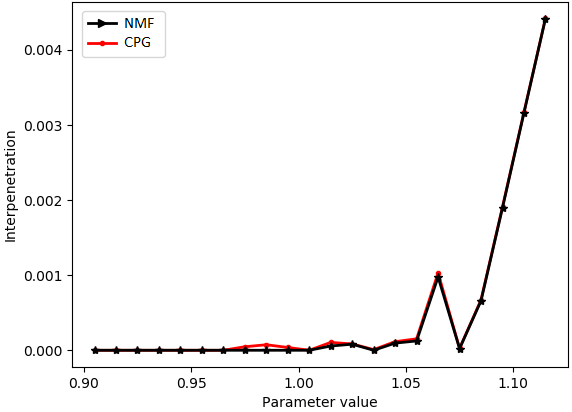
\includegraphics[width=.45\textwidth]{./images/contact/interp_second.png}
		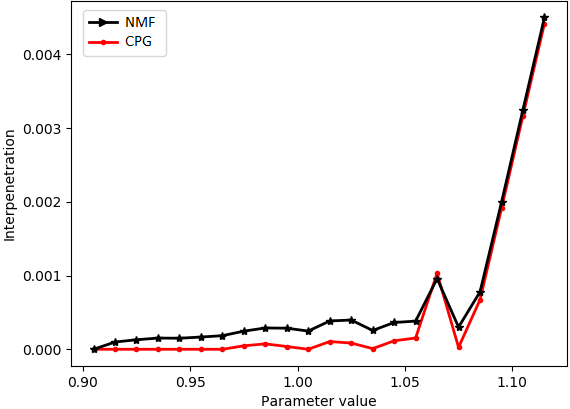
\includegraphics[width=.45\textwidth]{./images/contact/interp_third.png}
	\end{center}
	\begin{center}
		\small{ CPG/NMF(18)\hspace{2.8cm} CPG/NMF(5)}
	\end{center}
\end{frame}


\subsection{Ring on block}
\begin{frame}\frametitle{Ring on block}
	\begin{itemize}
		\item Imposed displacement at the ring's top ends
		\item Parametric ring's radius $\mu\in\mathcal P:=[0.95,1.15]$,
		$\mathrm{card}(\mathcal P^{\mathrm{tr}})=21$
		\item Non-matching meshes, \bl{$\mathcal N=2{\times}1590$} dofs, \ma{$\mathcal R = 50$ dofs}
		\item Reference (left) and deformed (right) configuration
	\end{itemize}
	\begin{center}
		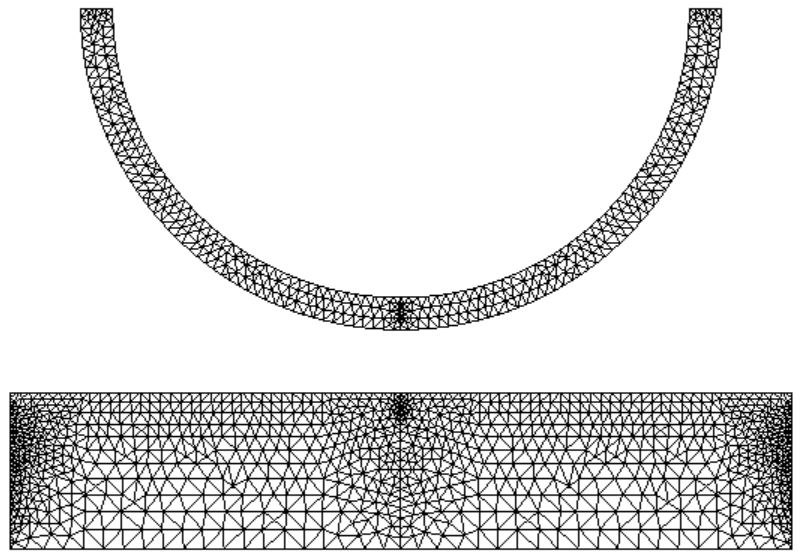
\includegraphics[width=0.4\textwidth]{./images/contact/ref_mesh.png}\quad
		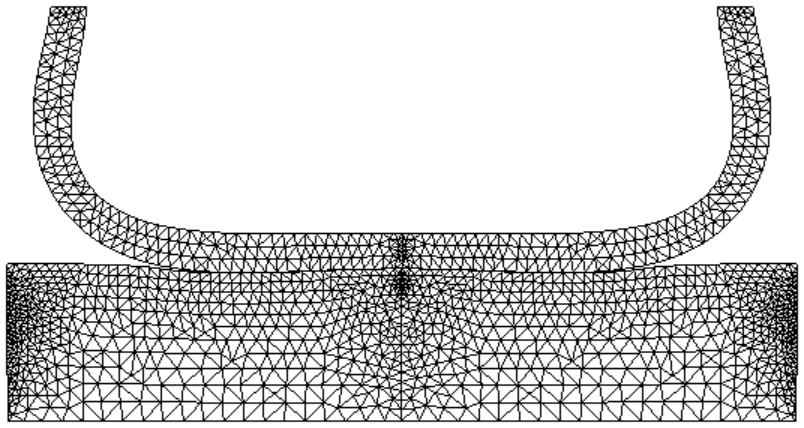
\includegraphics[width=0.4\textwidth]{./images/contact/def_mesh_1,1.png}
	\end{center}
\end{frame}

\begin{frame}\frametitle{Ring on block}
	Basis construction
	\begin{center}
		\hspace{-.7cm}
		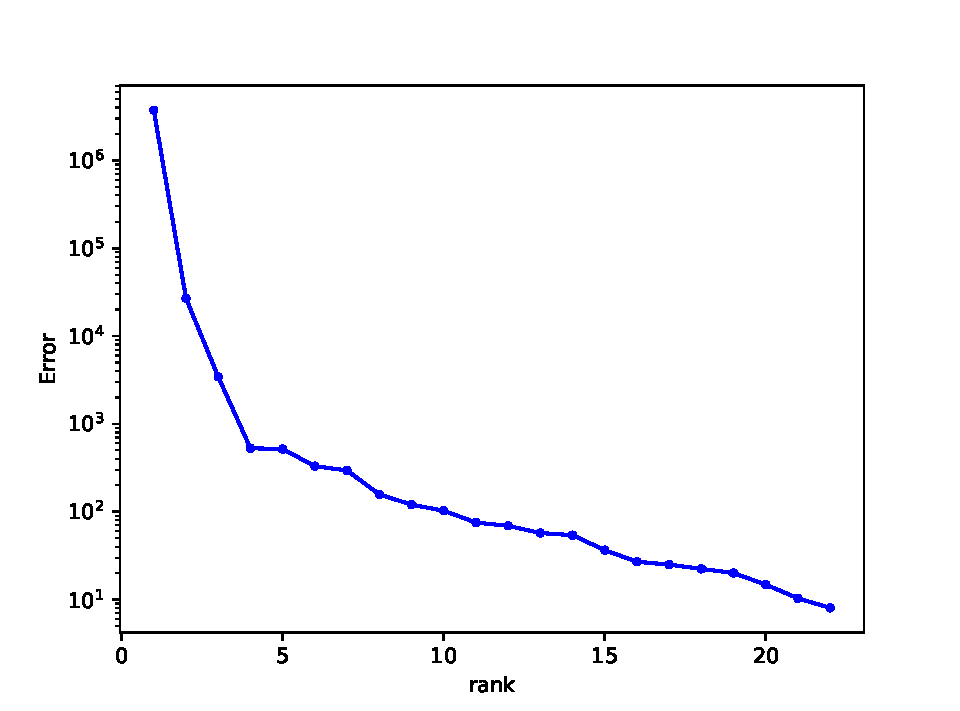
\includegraphics[width=.55\textwidth]{./images/contact/sgv_ring.pdf}
		\hspace{-.7cm}
		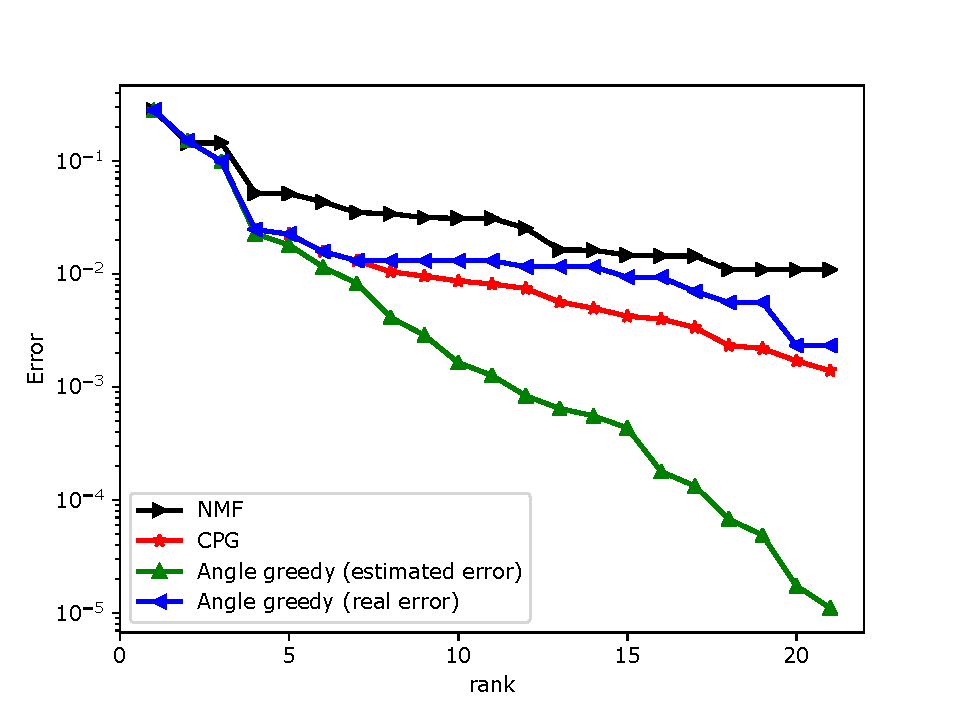
\includegraphics[width=.55\textwidth]{./images/contact/nmf_ring.pdf}
		\small{\hspace{1.8cm} \bl{Primal}basis
			\hspace{3.4cm} \ma{Dual}basis}
	\end{center}
\end{frame}

% \begin{frame}\frametitle{Ring on block}
	% \begin{itemize}
		% \item We take $N=21$ and $R=8$
		% % \item EIM on nonlinear gap functions ($M^k=20$, $M^g=21$)
		% \item $H^1$-displacement error
		% \end{itemize}
	% \begin{center}
		% 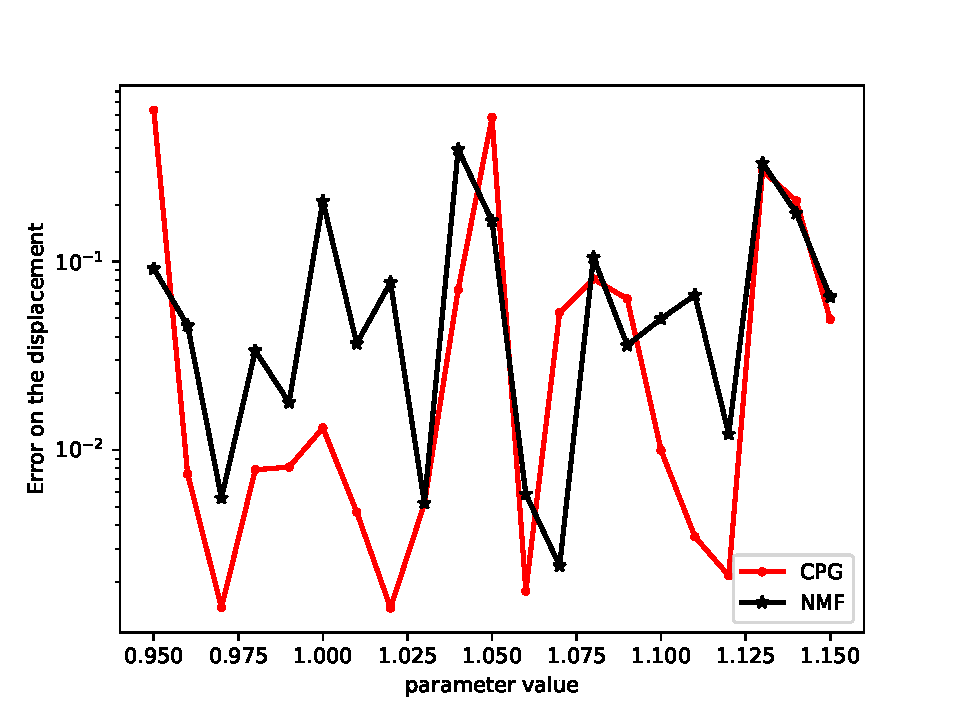
\includegraphics[width=.48\textwidth]{./images/contact/displ_ring.pdf}
		% 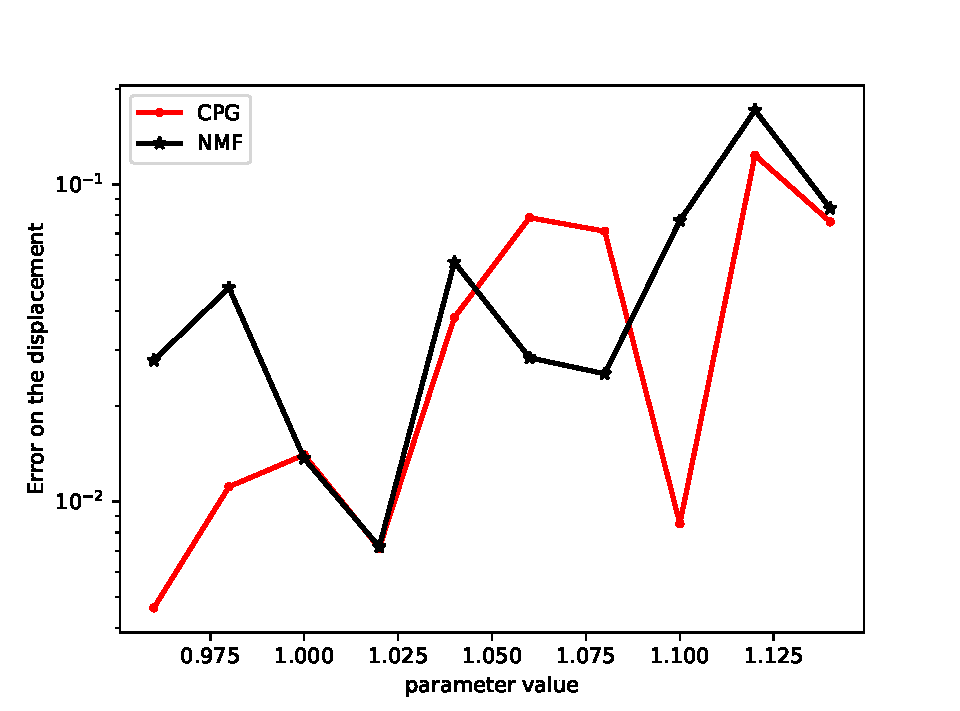
\includegraphics[width=.48\textwidth]{./images/contact/valid_displ_ring.pdf}
		% \end{center}
	% \small{\hspace{2cm} in training set\hspace{2.8cm}zoom in larger set}
	% \end{frame}


\section{}
\begin{frame}\frametitle{Conclusions and perspectives}
	\label{lastframe}
	\medskip
	
	\begin{columns}
		\begin{column}{.6\textwidth}
			{\bfseries Contributions}
			\begin{itemize}
				\item[{\gr\bfseries \cmark}] RBM in a general setting
				\begin{itemize}
					\item varying normals
					\item non-matching meshes
				\end{itemize}
				\item[{\gr\bfseries \cmark}] Cone-projected greedy algorithm 
				\begin{itemize}
					\item outperforms the NMF
					\item outperforms the angle-greedy
				\end{itemize}
			\end{itemize}
			
			{\bfseries Prespectives}
			\begin{itemize} 
				\item[{\red\bfseries ?}] Extensions to other types of contact
				\begin{itemize} 
					\item friction 
					\item multibody 
					\item dynamic 
				\end{itemize}
				\item[{\red\bfseries ?}] Convergence rates of the CPG
			\end{itemize}
		\end{column}
		\hspace{-1.4cm}
		
		\begin{column}{.5\textwidth}
			\begin{figure}
				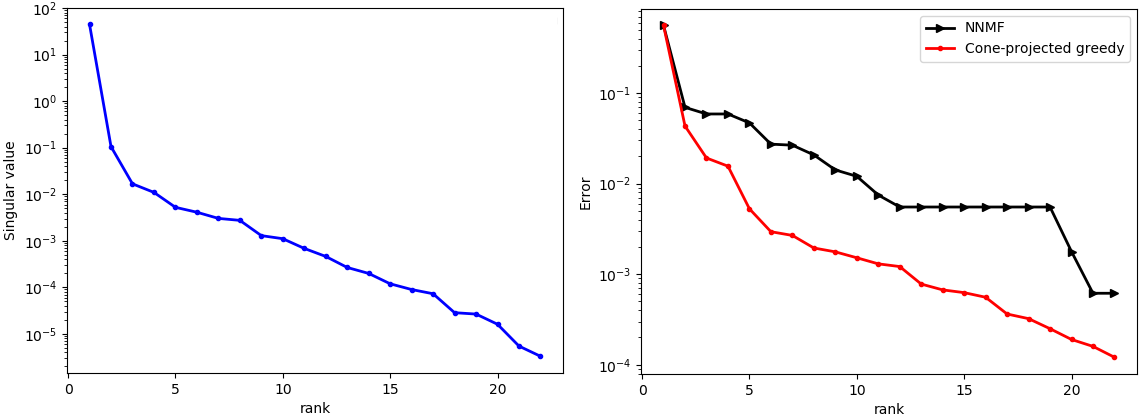
\includegraphics[trim=10.05cm 0cm 0cm 0cm, clip=true, width=.95\textwidth, angle=0]{./images/contact/sgv_nmf.png}
				\centering
			\end{figure}
		\end{column}
	\end{columns}
	
	\bigskip
	
	\medskip
	
	\mbox{
		\begin{minipage}{\textwidth}
			\begin{thebibliography}{1}
				\item {\footnotesize \textit{\bl{A reduced basis method for parametrized variational inequalities applied to contact mechanics.}}AB, V. Ehrlacher and A. Ern.  \textit{\bl{IJNME, 2019.}}}
			\end{thebibliography}
		\end{minipage}
	}
	\vspace{.6cm}
	
	% \begin{center}
		%  \quad\ \ \bfseries \large{\gr{Thank you for your attention}}
		% \end{center}
	
\end{frame}
